\label{result_positioning}

\subsubsection{Kết quả thực nghiệm}

\begin{table}[b!]
    \centering
    \caption{Số lượng cửa sổ dữ liệu hướng di chuyển trong NCV trên tập riêng tư}
    \label{nested_cv_direction}
    \begin{tabular}{llrr}\hline\hline
        \textbf{Vòng lặp ngoài (10 fold)} & \textbf{Vòng lặp trong (10 fold)} &  & \textbf{Tổng}\\\hline
        \multirow{2}{*}{Huấn luyện} & Huấn luyện & 2.563 & \multirow{2}{*}{2.848}\\\cline{2-3}
         & Xác thực & 285 & \\\hline
        Kiểm tra &  &  & 317\\\hline
        Tổng &  &  & 3.165\\\hline\hline
    \end{tabular}
\end{table}

\begin{figure}[b!]
    \centering
    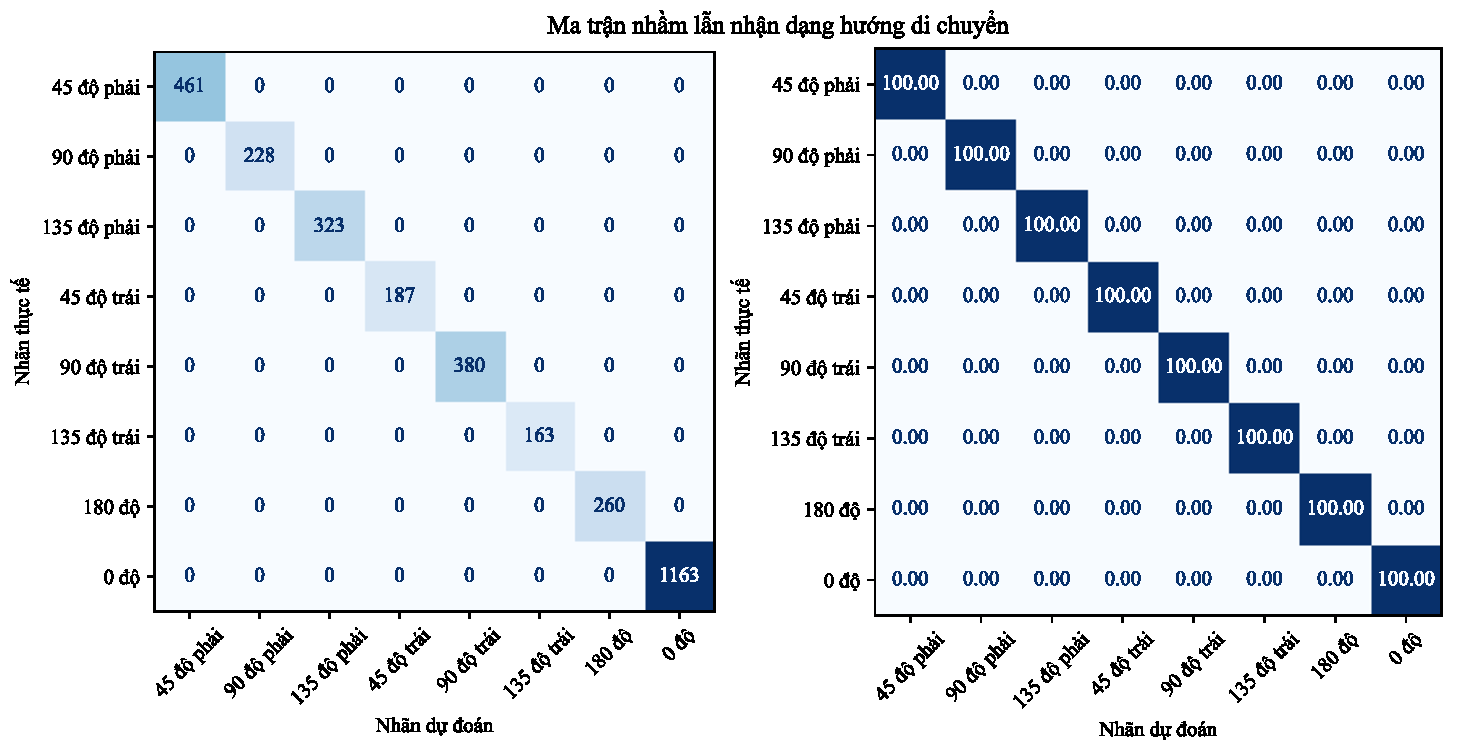
\includegraphics[width=1\linewidth]{Figure/confusion_matrix_direction.pdf}
    \caption{Ma trận nhầm lẫn nhận dạng hướng di chuyển}
    \label{confusion_matrix_direction}
\end{figure}

Để đánh giá hiệu suất của mô hình nhận dạng hướng di chuyển, phương pháp NCV đã được áp dụng nhằm ước lượng sai số tổng quát một cách đáng tin cậy. Cụ thể, kỹ thuật StratifiedKFold được sử dụng trong cả vòng lặp ngoài và vòng lặp trong để xử lý vấn đề mất cân bằng phân bố giữa các lớp dữ liệu. Vòng ngoài gồm 10 fold được sử dụng để đánh giá mô hình, trong khi vòng trong cũng gồm 10 fold nhằm xác định bộ siêu tham số tối ưu cho từng lần lặp ngoài.

Tổng số phân đoạn dữ liệu huấn luyện, xác thực và kiểm tra trong quy trình NCV được trình bày chi tiết trong bảng~\ref{nested_cv_direction}. Quy trình NCV đảm bảo rằng tập kiểm tra hoàn toàn độc lập với tập huấn luyện và xác thực, từ đó giúp giảm thiểu nguy cơ quá khớp và nâng cao độ tin cậy của kết quả. Sau khi hoàn tất quá trình lựa chọn siêu tham số, mô hình được tinh chỉnh thêm bằng quy trình VCV nhằm tối ưu hóa hiệu suất phân loại trên toàn bộ tập dữ liệu huấn luyện.

Mô hình học máy được lựa chọn cuối cùng là DT với độ sâu tối ưu bằng 6 và kích thước bộ nhớ chỉ 3,34 kB. Kết quả phân loại trên toàn bộ cơ sở dữ liệu hướng di chuyển được thể hiện qua ma trận nhầm lẫn trong hình~\ref{confusion_matrix_direction}. Đáng chú ý, mô hình đạt độ chính xác phân loại tuyệt đối $100\%$ trên các lớp hướng di chuyển.

Về mặt tài nguyên triển khai, mô hình có kích thước nhỏ hơn 1 MB, phù hợp với giới hạn bộ nhớ của nhiều vi điều khiển phổ biến hiện nay. Điều này cho thấy rằng các mô hình học máy nhẹ như DT là lựa chọn khả thi cho các ứng dụng nhúng trong thời gian thực, đặc biệt là trong các hệ thống hỗ trợ chiến sĩ cứu hộ, nơi yêu cầu xử lý nhanh với độ trễ thấp và độ tin cậy cao. Việc nhận dạng chính xác hướng di chuyển không chỉ góp phần nâng cao độ chính xác tổng thể của hệ thống định vị, mà còn có ý nghĩa đặc biệt trong việc hỗ trợ giám sát và đảm bảo an toàn cho chiến sĩ trong các tình huống khẩn cấp và môi trường phức tạp.

\begin{figure}[b!]
    \centering
    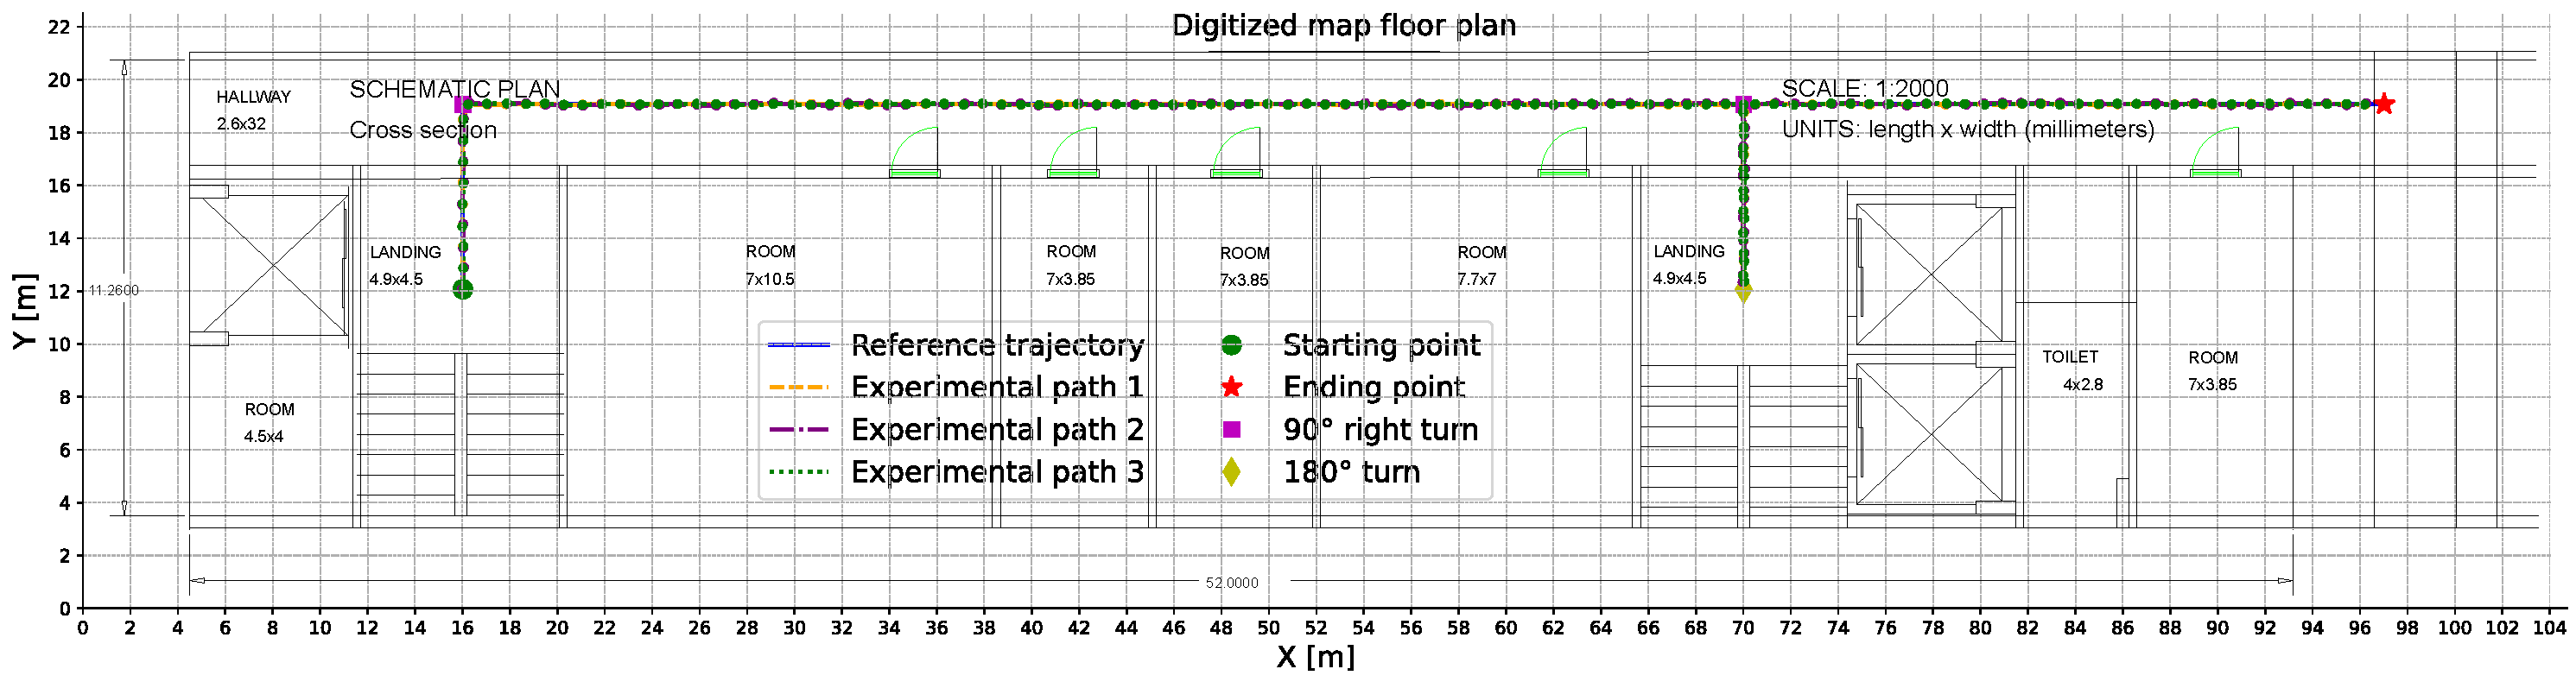
\includegraphics[width=1\linewidth]{Figure/schematic_plane_cross_bold.pdf}
    \caption{Bản đồ số hóa với quỹ đạo tham chiếu và thực nghiệm}
    \label{schematic_plane_cross_bold}
\end{figure}

\begin{table}[b!]
    \centering
    \caption{Khoảng cách ước tính và lỗi trong năm lần thử nghiệm (180 bước, khoảng cách thực tế = 101,5~m)}
    \label{experiment_distance}
    \begin{tabular}{lrrrrr} \hline\hline
    \textbf{Số lần thử nghiệm} & \textbf{1} & \textbf{2} & \textbf{3} & \textbf{4} & \textbf{5} \\ \hline
    Quãng đường ước tính (m) & 101,99 & 102,23 & 101,93 & 102,39 & 100,79\\
    Sai số (m) & 0,49 & 0,73 & 0,43 & 0,89 & 0,71\\ \hline\hline
    \end{tabular}
\end{table}

Trong nghiên cứu này, phương pháp ước tính quãng đường di chuyển được thực hiện dựa trên sự kết hợp giữa bộ đếm bước và phép đo khoảng cách liên chi thông qua LiDAR. Hình ảnh mặt bằng số hóa (Hình~\ref{schematic_plane_cross_bold}) được sử dụng để thiết lập tuyến đường thực nghiệm với kích thước thực tế là 104~m chiều dài và 22,52~m chiều rộng. Để đánh giá độ tin cậy của bộ lọc đa giai đoạn trong việc loại bỏ các vật thể ngoài ý muốn (ví dụ: bức tường, đồ vật), các thử nghiệm được thực hiện trong một hành lang có chiều rộng 2~m, với hai bên là các bức tường. Mỗi lần thử nghiệm bao gồm 180 bước chân, với quãng đường thực tế tương ứng là 101,5~m. Kết quả thực nghiệm cho thấy mô hình ước tính độ dài bước đạt sai số tuyệt đối trung bình 5 cm và độ lệch chuẩn 4,36 cm trên mỗi bước, qua đó đảm bảo tính chính xác của phương pháp ước tính quãng đường di chuyển. Bên cạnh đó, kết quả ước tính quãng đường di chuyển cho từng lần thử nghiệm được trình bày chi tiết trong bảng~\ref{experiment_distance}. Cụ thể, khoảng cách ước tính dao động từ 100,79~m đến 102,39~m, với sai số dao động từ 0,43~m đến 0,89~m. Đáng chú ý, sai số định vị tổng thể của hệ thống luôn duy trì dưới 2~m trong tất cả các thử nghiệm, khẳng định tính hiệu quả và độ tin cậy của phương pháp đề xuất. Điều này là một lợi thế quan trọng đối với các ứng dụng trong môi trường cứu hộ khẩn cấp trong nhà, nơi yêu cầu cao về tính chính xác và khả năng theo dõi liên tục.

Tuy nhiên, phương pháp ước tính quãng đường di chuyển sử dụng LiDAR chỉ thực sự khả thi trong các trạng thái di chuyển đi bộ hoặc đi nhanh—tức là khi đối tượng di chuyển đều và luôn có ít nhất một chân chạm đất. Trong trường hợp đối tượng chuyển sang trạng thái chạy bộ, cả hai chân có thể đồng thời không chạm đất, dẫn đến gián đoạn trong phép đo khoảng cách của LiDAR. Do đó, trong tình huống chạy bộ, hệ thống chỉ có thể dựa vào bộ đếm bước để ước tính quãng đường di chuyển, trong khi các phép đo từ LiDAR có thể bị loại bỏ hoặc không đáng tin cậy do sự bất ổn định trong dữ liệu quét. Nhìn chung, các kết quả thực nghiệm đã chứng minh tính khả thi và hiệu quả của phương pháp tích hợp LiDAR và bộ đếm bước trong việc ước tính quãng đường di chuyển của đối tượng trong môi trường trong nhà. Tuy nhiên, để mở rộng ứng dụng cho các tình huống phức tạp hơn như chạy bộ, bò trườn, cần có các phương pháp hiệu chỉnh và điều chỉnh thuật toán nhằm đảm bảo tính chính xác và ổn định của hệ thống.

\subsubsection{Thảo luận các phương pháp định vị nhân viên cứu hộ trong nhà}

\begin{figure}[t]
    \centering
    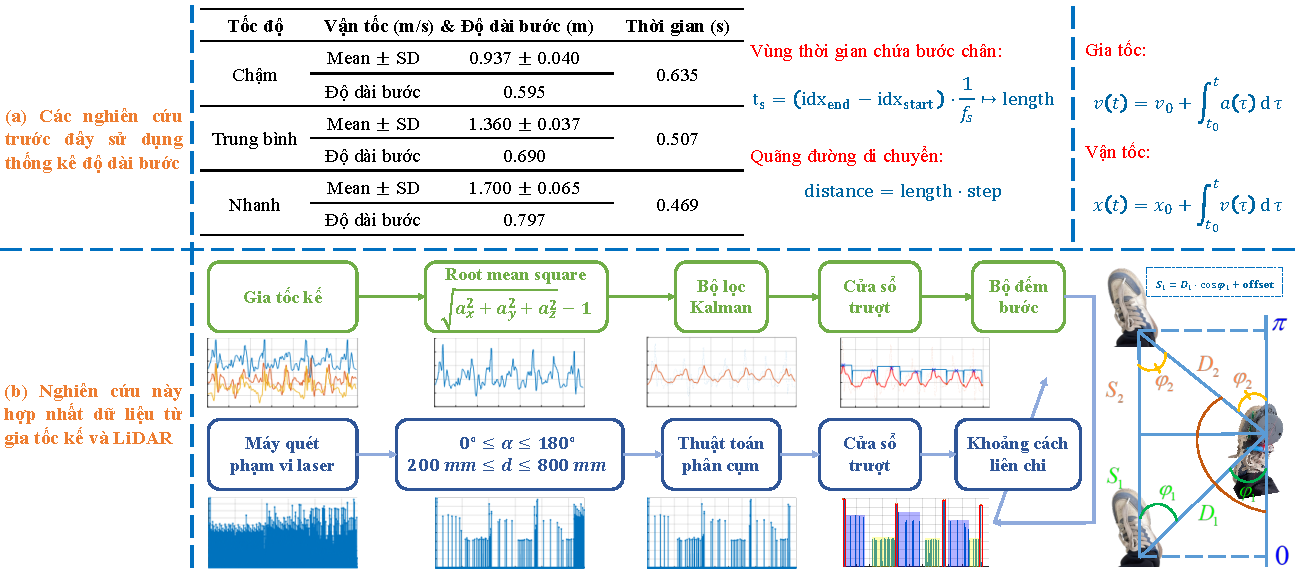
\includegraphics[width=1\linewidth]{Figure/discussion_ips.pdf}
    \caption{So sánh giữa (a) Phương pháp ước lượng quãng đường di chuyển dựa trên thống kê độ dài bước trong các nghiên cứu trước đây~\cite{pham2018highly}, \cite{ho2016step} và (b) Chiến lược hợp nhất cảm biến IMU-LiDAR đề xuất trong nghiên cứu này}
    \label{discussion_estimate}
\end{figure}

Trong các nghiên cứu trước đây, việc ước tính quãng đường di chuyển thường dựa vào việc đếm số bước kết hợp với bảng tra thống kê độ dài bước tương ứng với từng mức tốc độ (chậm, trung bình, nhanh)~\cite{pham2018highly}, \cite{ho2016step}. Phương pháp này giả định rằng độ dài bước chân là hằng số đối với mỗi người tại mỗi tốc độ, từ đó nhân với số bước để tính quãng đường (Hình~\ref{discussion_estimate}a). Tuy nhiên, giả định này khó phản ánh chính xác chuyển động thực tế vì độ dài bước phụ thuộc vào nhiều yếu tố như thể trạng, dáng đi, tải trọng mang theo, trạng thái mệt mỏi hoặc đặc thù thao tác của lính cứu hỏa trong điều kiện khẩn cấp.

Nhằm khắc phục nhược điểm trên, nghiên cứu này đề xuất một phương pháp hợp nhất dữ liệu từ cảm biến quán tính (IMU) và máy quét phạm vi laser (LiDAR) thông qua một kiến trúc bộ lọc đa giai đoạn, nhằm ước lượng chính xác quãng đường di chuyển theo thời gian thực (Hình~\ref{discussion_estimate}b). Cụ thể, bộ đếm bước sử dụng tín hiệu gia tốc từ IMU giúp xác định chính xác thời điểm diễn ra từng bước chân. Thông tin này đóng vai trò là tín hiệu khởi phát cho thuật toán phát hiện đỉnh từ dữ liệu LiDAR, vốn được xử lý qua ba tầng lọc: giới hạn phạm vi quét, phân cụm để loại bỏ nhiễu, và cửa sổ trượt để phát hiện đỉnh tương ứng với khoảng cách giữa hai bàn chân.

Cách tiếp cận này mang lại hai lợi ích quan trọng. Thứ nhất, nó loại bỏ được các bước chân giả do dao động nhiễu hoặc vật thể ngoài vùng quan tâm trong dữ liệu LiDAR. Thứ hai, nó đảm bảo rằng chỉ các bước chân hợp lệ mới được đưa vào tính toán, từ đó giúp cải thiện độ chính xác trong ước lượng độ dài bước. Việc sử dụng thông tin đo trực tiếp thay vì dựa trên bảng tra cứu giúp hệ thống thích ứng linh hoạt với hành vi chuyển động thực tế của từng cá nhân trong nhiều tình huống khác nhau—điều đặc biệt quan trọng trong môi trường khẩn cấp như tìm kiếm cứu nạn. Tóm lại, phương pháp đề xuất không chỉ cải thiện độ chính xác định vị so với cách tiếp cận truyền thống mà còn có tính thích nghi cao và khả năng ứng dụng thực tiễn trong các kịch bản khắc nghiệt. Hệ thống cho thấy tiềm năng lớn trong việc hỗ trợ giám sát và điều phối chiến sĩ cứu nạn trong các tòa nhà bị ảnh hưởng bởi hỏa hoạn, nơi các công nghệ định vị dựa trên hạ tầng gần như không thể hoạt động ổn định.

\begin{table}[t]
    \centering
    \caption{So sánh các phương pháp định vị nhân viên cứu hộ trong nhà tiêu biểu cho các tình huống khẩn cấp}
    \label{discussion_ips}
    \begin{tabular}{p{0.09\linewidth}p{0.151\linewidth}p{0.2\linewidth}p{0.186\linewidth}p{0.24\linewidth}}\hline\hline
        \multicolumn{1}{c}{\textbf{Ấn phẩm}} & \multicolumn{1}{c}{\textbf{Công nghệ}} & \multicolumn{1}{c}{\textbf{Phương pháp}} & \multicolumn{1}{c}{\textbf{Kỹ thuật}} & \multicolumn{1}{c}{\textbf{Sai số và thách thức}}\\\hline

        \multirow{8}{*}{\parbox[t]{\linewidth}{\justifying \noindent Nghiên cứu này}} & \multirow{8}{*}{\parbox[t]{\linewidth}{\justifying \noindent IMU 6-DoF, khí áp kế (thắt lưng) và LiDAR (bàn chân)}} & \makecell[tl]{\parbox[t]{\linewidth}{\justifying \noindent - IMU đếm bước + sải chân từ LiDAR giữa các chân.\\- 8 lớp HAR và 8 lớp di chuyển.\\- Ước tính độ cao từ khí áp kế kết hợp IMU và HAR.}} & \multirow{8}{*}{\makecell[tl]{\parbox[t]{\linewidth}{\justifying \noindent - Lọc LiDAR 3 giai đoạn.\\- XGBoost cho HAR.\\- DT cho hướng di chuyển.\\- Bộ lọc Kalman.}}} & \multirow{8}{*}{\makecell[tl]{\parbox[t]{\linewidth}{\justifying \noindent - HAR 98,38~\%, hướng di chuyển 100~\%.\\ - Lỗi định vị $<$ 2~m.\\- Ổn định trong trạng thái đi bộ.\\ - Tắc nghẽn LiDAR, biến đổi áp suất.}}} \\
        \hline
        
        \multirow{6}{*}{\makecell[tl]{Yuan \\ \textit{et al.}~\cite{yuan2016research}}} & \multirow{6}{*}{\parbox[t]{\linewidth}{\justifying \noindent IMU 6-DoF (bàn chân)}} & \multirow{6}{*}{\makecell[tl]{\parbox[t]{\linewidth}{\justifying \noindent - Tính khoảng cách và độ cao bằng gia tốc kế.\\- Xác định hướng bằng con quay hồi chuyển.}}} & \multirow{6}{*}{\makecell[tl]{\parbox[t]{\linewidth}{\justifying \noindent - Tích phân kép INS: \\ $p_n = \int v_n\,dt = \int (a_n + g_t)\,dt$.\\- Tối ưu hóa rời rạc và ZUPT.}}} & \makecell[tl]{\parbox[t]{\linewidth}{\justifying \noindent - Sai số tương đối $<$ 1~\% (sai số tuyệt đối lên tới 2,5~m).\\- Độ trôi tích lũy theo thời gian.\\- Biến thiên dáng đi.}} \\
        \hline
        
        \multirow{10}{*}{\makecell[tl]{Cinaz và \\ Kenn~\cite{cinaz2008headslam}}} & \multirow{10}{*}{\parbox[t]{\linewidth}{\justifying \noindent IMU 6-DoF và máy quét laser (gắn đầu)}} & \multirow{10}{*}{\makecell[tl]{\parbox[t]{\linewidth}{\justifying \noindent - Định vị và lập bản đồ đồng thời (SLAM).\\- Laser quét hiệu chỉnh theo hướng đầu (IMU).\\- Vận tốc bước giả định từ IMU.}}} & \multirow{10}{*}{\makecell[tl]{\parbox[t]{\linewidth}{\justifying \noindent - Bộ lọc hạt Rao-Blackwellized (GMapping).\\- Ước lượng bước từ dao động trục Z.\\- Biến đổi góc 3D thành mặt phẳng quét.}}} & \makecell[tl]{\parbox[t]{\linewidth}{\justifying \noindent - 0,7~m trong phòng có vật cản.\\- 6 đến 12~m trong hành lang mở.\\- 18~m trong hành lang trống.\\- Phụ thuộc đặc trưng môi trường.\\- Lỗi do chuyển động đầu phức tạp.}} \\
        \hline
        
        \multirow{5}{*}{\makecell[tl]{De \\ \textit{et al.}~\cite{de2017hybrid}}} & \multirow{5}{*}{\parbox[t]{\linewidth}{\justifying \noindent IMU 9-DoF (thắt lưng) và thẻ RFID thụ động}} & \makecell[tl]{\parbox[t]{\linewidth}{\justifying \noindent - IMU ước lượng chuyển động.\\- RFID sửa lỗi trôi.\\- RFID cài sẵn trong đèn báo khẩn cấp.}} & \makecell[tl]{\parbox[t]{\linewidth}{\justifying \noindent - Vi phân quaternion: \\ $\frac{d\mathbf{q}}{dt} = \boldsymbol{\Omega} \mathbf{q}$.\\- Bộ lọc định hướng Kalman mở rộng.\\ - Bộ lọc Bayesian.}} & \multirow{5}{*}{\makecell[tl]{\parbox[t]{\linewidth}{\justifying \noindent - Sai số $<$ 4~m với PDR; $<$ 2.6~m với hệ lai.\\- Từ kế bị nhiễu.\\- Thẻ RFID có thể hư hỏng.}}} \\\hline\hline
    \end{tabular}
\end{table}

Bên cạnh các phương pháp thống kê truyền thống trong ước lượng quãng đường, nhiều nghiên cứu trong lĩnh vực định vị lính cứu hỏa cũng khai thác các kỹ thuật cảm biến đeo không phụ thuộc hạ tầng để đảm bảo tính tự chủ và khả năng triển khai trong môi trường khẩn cấp. Bảng~\ref{discussion_ips} định vị cách tiếp cận của chúng tôi so với các phương pháp định vị trong nhà tiêu biểu gồm: định vị quán tính thuần túy, định vị dựa trên SLAM với máy quét laser đeo đầu, và định vị lai IMU-RFID.

Yuan \textit{et al.}~\cite{yuan2016research} đề xuất một hệ thống định vị độc lập hoàn toàn dựa trên IMU gắn ở bàn chân, kết hợp thuật toán phát hiện bước, ước lượng vận tốc và hiệu chỉnh bằng kỹ thuật ZUPT. Nhờ xác định chính xác thời điểm chân đứng yên, hệ thống có thể hạn chế sai số tích lũy khi tích phân vận tốc. Thử nghiệm thực tế với các tình huống đa dạng (đi bộ, chạy, leo cầu thang, địa hình đổ nát) cho thấy sai số tương đối thấp (khoảng $<$ 1~\%, sai số tuyệt đối lên đến 2,5~m) trên các hành trình ngắn và vừa. Tuy nhiên, khi kéo dài thời gian hoạt động, hệ thống vẫn gặp vấn đề với trôi tích lũy, đặc biệt trong điều kiện không có thông tin hiệu chỉnh từ bản đồ hay hạ tầng. Ngoài ra, hướng chuyển động dễ bị sai lệch nếu không có hỗ trợ từ cảm biến từ trường hoặc các mô hình bổ sung.

Cinaz và Kenn~\cite{cinaz2008headslam} với hệ thống HeadSLAM kết hợp IMU và máy quét laser gắn trên đầu nhằm thực hiện đồng thời định vị và lập bản đồ môi trường 2D thông qua thuật toán SLAM dựa trên bộ lọc hạt Rao-Blackwellized. Phương pháp này có ưu điểm lớn là không phụ thuộc vào bản đồ có sẵn hay hạ tầng định vị, đồng thời tận dụng kỹ thuật scan matching để tăng cường khả năng xác định vị trí trong thời gian thực. Tuy nhiên, sai số định vị tăng đáng kể trong môi trường hành lang đơn điệu hoặc không có vật cản đặc trưng, với độ lệch có thể lên đến 18~m (cụ thể 0,7~m trong phòng có vật cản, 6 đến 12~m trong hành lang mở, 18~m trong hành lang trống). Hạn chế chủ yếu nằm ở việc quét laser bị ảnh hưởng mạnh bởi hướng chuyển động đầu, chuyển động holonomic không ổn định, và không có cơ chế đóng vòng hiệu quả—điều vốn rất quan trọng trong các hành trình dài hoặc khép kín.

De Cillis \textit{et al.}~\cite{de2017hybrid} đề xuất hệ thống lai IMU-RFID với chiến lược hiệu chỉnh vị trí dựa trên thông tin định vị tích hợp trong thẻ RFID cài sẵn tại các vị trí chiến lược trong tòa nhà. Với thiết kế bộ lọc Bayes hai pha: pha dự đoán dựa trên bước đi PDR từ dữ liệu quán tính và pha hiệu chỉnh dựa trên thông tin ngữ cảnh được trích xuất từ thẻ RFID gắn sẵn tại các vị trí chiến lược, hệ thống có thể duy trì sai số định vị dưới 2,6~m kể cả trong hành trình kéo dài, miễn là thẻ RFID không bị phá hủy hoặc mất tín hiệu và dưới 4~m chỉ với PDR. Tuy vậy, việc phụ thuộc vào các nút RFID khiến hệ thống dễ bị ảnh hưởng nếu thẻ bị hỏng, lắp sai hoặc không đủ mật độ phủ. Bên cạnh đó, không giống như cảm biến gắn ở bàn chân, IMU gắn thắt lưng không cho phép áp dụng các kỹ thuật ZUPT, từ đó làm tăng rủi ro tích lũy sai số khi di chuyển liên tục mà không có hiệu chỉnh.

So với các nghiên cứu trên, phương pháp đề xuất trong nghiên cứu này lựa chọn chiến lược hợp nhất IMU-LiDAR với kiến trúc lọc ba tầng, đồng thời khai thác vị trí lắp đặt cảm biến hợp lý (IMU tại thắt lưng và LiDAR tại bàn chân phải) để trực tiếp đo khoảng cách giữa hai chân—qua đó tính toán độ dài bước trong thời gian thực thay vì dựa vào bảng thống kê. Cách tiếp cận này không chỉ đảm bảo độ chính xác cao ($<$ 2~m) trong hành trình tuyến tính mà còn cải thiện khả năng thích nghi với thay đổi tư thế, sải chân và trạng thái hoạt động của lính cứu hỏa. Hệ thống cũng cho thấy khả năng triển khai thực tế cao nhờ kích thước mô hình nhỏ, dễ nhúng và không yêu cầu bất kỳ hạ tầng bên ngoài nào. Nhờ đó, phương pháp đề xuất đã khắc phục được hạn chế quan trọng của các nghiên cứu trước: hoặc chưa có biện pháp hiệu chỉnh sai số tích lũy theo thời gian (Yuan \textit{et al.}~\cite{yuan2016research}), hoặc phụ thuộc vào môi trường (HeadSLAM~\cite{cinaz2008headslam}, De Cillis \textit{et al.}~\cite{de2017hybrid}).

Tổng thể, sự kết hợp giữa đặc trưng động học từ IMU, phép đo vật lý chính xác từ LiDAR, và bộ lọc đa tầng xử lý dữ liệu đầu vào, đã giúp hệ thống đề xuất trở thành một giải pháp cân bằng giữa độ chính xác, tính tự chủ và khả năng triển khai trong môi trường nguy hiểm, vốn là yêu cầu cốt lõi trong bài toán định vị lính cứu nạn trong nhà. Những lợi ích bắt nguồn từ ước tính bước chân LiDAR giữa các chân và khí áp kế hỗ trợ độ cao, giúp hạn chế độ trôi mà không cần đèn hiệu môi trường. Các hạn chế bao gồm tắc nghẽn LiDAR và các biến đổi áp suất; công việc trong tương lai sẽ nhắm mục tiêu vào các đường dẫn dài hơn, các đoạn rẽ gấp và chuyển đổi nhiều tầng thông qua sự kết hợp mạnh mẽ hơn.
